\documentclass[letterpaper]{article}
\usepackage{natbib, alifexi}
\usepackage{amssymb}
\usepackage{amsmath}
\usepackage[formats]{listings}
\usepackage{xcolor}

\pagestyle{plain}
\setlength{\footskip}{30pt}

\renewcommand{\lstlistingname}{Implementation}
\renewcommand{\ttdefault}{pcr}
\lstdefinelanguage{CustomPy}{
	language=Python,
	basicstyle=\ttfamily\footnotesize\bfseries,
	linewidth=\linewidth,
    keywordstyle=\color{green!60!black},
	morekeywords=[2]{occurEvent,newTheta,minColor,setRelevance,keepHigherPower,getPower,sendMsg,clear},
	keywordstyle={[2]\color{blue}},
    identifierstyle=\color{black},
    flexiblecolumns=true,
	resetmargins=true,
    tabsize=2,
    showtabs=false,
    breaklines=true,
	breakatwhitespace=true,
	breakautoindent=true,
    captionpos=b,
    frame=tb,
    framerule=0.75pt,
    numbers=left,
    numberstyle=\scriptsize\color{gray!75!black}
}

\title{Distributed Graph Coloring}
\author{Xavier Barthel, Maxime Godfroid \and Quentin-Emmanuel Vajda \\
\mbox{}\\
ULB}

\begin{document}
\maketitle

\begin{abstract}
The graph coloring problem is to assign a color to each node of a graph such as no neighboring nodes have the same color ; and while maintaining as few colors as possible. The need of efficient algorithms capable of solving this problem is great. In this paper, some of the stat of the art heuristics in both centralized and distributed systems used to solve said problem are summarized. The main subject is the algorithm called \emph{FrogSim} which is based on the behaviour of Japanese tree frogs. This algorithm and its implementation is explained in great details. Data resulting from an array of test performed on both random geometric graphs and grid topologies are also discussed. Finally a few possible improvements thought of during our researches of this subject are presented.
\end{abstract}

\section{Introduction}
\subsection{Graph Coloring}
Graph coloring is a problem involving the coloration of a given graph ; each node of said graph has a certain color assigned to it. A valid coloring is found when all neighboring nodes\footnote{All the nodes with which a given node has a common link.} have different colors.\\

The graph coloring problem is to verify if a given graph can be colored using $k$ different colors and to find said coloration\footnote{Or a coloration using less than $k$ colors.} if it exists.\\

Based on the above, the $k^*$ minimum number of colors necessary for a given graph is determined and the optimal coloration is found.

\subsubsection{Usage}
One of the most well known usage of non-centralized algorithm to solve graph coloring instances is the channel assignment in wireless networks. The radio emitters are represented as the nodes in the graph. A color corresponds to a radio frequency used by a emitter. the coupling of color with node is needed to reduce the interferences and thus enhance the stability of the network. The topology of wireless networks is often similar to a grid or geometric graph, which are both described further.

\subsubsection{Centralized}
Centralized algorithm to solve the graph coloring problem have existed, been studied and improved for a few decades. The following are some of the most well known of these algorithms.

\paragraph{Deterministic}
The graph coloring problem is what is called a "\emph{NP-Hard problem}", a non-deterministic polynomial algorithm for which no deterministic algorithm performing with polynomial complexity is known. This leads to the computational infeasibility to solve the problem at hand using a deterministic algorithm.\\

This does not mean that no deterministic algorithm solving this problem exist however. But it does mean that non of these algorithm are applicable in practice. For this reason, they will not be detailed here.\\

More information concerning deterministic algorithm ave been detailed by ~\cite{DeMarco2001FDG} and ~\cite{Barenboim2011DDV}.

\paragraph{(Meta-)Heuristic}
As discussed previously, the graph coloring problem is \emph{NP-Hard}, which means that there exists non-deterministic algorithm to solve it that will run in polynomial time. These algorithms are often referred to as heuristic or meta-heuristic when used in practice.\\

Heuristics do not guarantee to find the optimal solution to a problem, nor to always give the same solution to a problem. This come from the random nature of their implementation, which itself comes from the non-determinism of the algorithm it represents.\\

Some example of heuristics capable of solving the graph coloring problem are presented here under. Most of these algorithm are based on general algorithm capable of solving most \emph{NP} problems ; as such they have common notions :

\begin{itemize}
\item A result ; for graph coloring, an association pairing each node to a color.
\item A transformation ; when applied to one or multiple result, it will yield a new result. Examples of such transformations in graph coloring could be to simply assign a new random color to a node of the given result, or swap the colors of two randomly picked nodes.
\end{itemize}

\paragraph{Evolutionary}
The general evolutionary algorithm is heavily inspired by the evolution of a population as studied in biology. The notions used are the idea that a population will evolve by reproduction,mutation and selection. These are the different transformations applied on a population composed of possible results to the problem.\\

An application of this heuristic to the graph coloring problem has been proposed by~\cite{Malaguti2008MAV}.

\paragraph{Tabu Search}
The very general principle of the Tabu search is to evolve from a valid solution and search for optimization by applying transformations. The idea is then to only apply transformations that will yield the best results and are not \emph{tabu} ; which means that they have not been applied recently.\\

This general algorithm as been specialized and optimized for the purpose of the graph coloring problem, notably by~\cite{Blochliger2008GCH}. The particularity of this heuristic is the decomposition of the global solution allocating a color to each node, in multiple sub-solutions giving colors to only a subset of nodes.

\paragraph{Genetic Local Search}
Detailed by ~\cite{Dorne98anew}, this algorithm is a hybrid approach to the graph coloring problem. Combining the global association of results set provided by the genetic heuristic, and the search for local optimization of the Tabu search, gives good results. In particular for the \emph{DIMACS} benchmarking graphs.

\paragraph{Variable Neighborhood}
The great performances of the variable space search proposed by ~\cite{hertz2008}, comes from its unique ideas. The main one being to find local optimizations in specific search spaces where global constraints are not guaranteed and to combine these optimizations to obtain a valid result for the whole problem.

\subsubsection{Distributed}
The graph coloring problem can be resolved in a centralized manner as previously explained. However, in practice most possible uses of graph coloring are in distributed systems.\\ 

The distributed approach depends on swarm intelligence where multiple agents all possessing only limited ressources\footnote{Computational ressources, memory, battery ...} work together to achieve a global goal. In the case of graph coloring problem, each node is a separate agent whose limited resources only allow to communicate with its direct neighbors. The common goal in this scenario is finding the optimal coloring.\\

Due to the constraints brought by distributed systems, namely the lack of ressources, the algorithms used here are much more specialized. Because this lack of ressources can be of many different nature a given problem can have many different heuristics solving it while optimizing each a different aspect. for instance, a distributed system whose main constraint is its real time nature will have algorithm designed around the idea of minimal time complexity whereas if the main constraint was the low computational power of each agent the same problem would be solved with an algorithm specialized to require less calculations.\\

The focused attributes of the following will be time complexity, calculation complexity as well as message load\footnote{The size of the messages exchanged by the different agent. The smaller it is the less time spent transfering information which in turn diminishes the energy required to operate.}.\\

Graph coloring also allows even more specialization because each topology of graphs can have an associated algorithm.\\

One of the most effective, while still being very general work, was produced by ~\cite{Finocchi2002EAS}. It presents three versions of an algorithm focusing on different constraints of distributed systems.\\

Another interesting heuristic was presented by~\cite{KubaleKuzner}. The DLF (\emph{Distributed Largest-First}) algorithm uses a random ordering of the nodes as well as a partial ordering based on the degree of each node\footnote{The degree of a node being the number of neighbors a node has.} to simplicitate and accelerate the process of picking a valid color for each agent.\\

This short and non-exhaustive list of different techniques can easily be extended. In fact, any techniques of artificial intelligence can reasonably easily and with varying degrees of success be adapted to fit the problem at hand. However we have here only presented a few chosen techniques that can be compared to the \emph{FrogSim} algorithm.\\

The heuristic based on the calling behaviour of the Japanese tree frog is the main subject of this paper. The main idea behind it is to emulate the anti-phase synchronization of said frogs to allow each node to discover its color as fast as possible while sending minimal messages. It is explained in greater details in the following sections.\\

This idea has been exploited in the past by~\cite{Lee2008EDP} and later refined by~\cite{Lee2010}. The \emph{FrogSim} algorithm, presented in the rest of this paper, is another improvement on these two techniques.

\section{Methods}
\subsection{Calling Behaviour Model}
This algorithm is based on the calling behaviour of Japanese tree frog. As said by~\cite{Aihara}, it has been observed that in the calling behavior of multiple males frogs interacting together, the anti-phase synchronization is stable and, if it occurs, the in-phase synchronization is transient. The male frogs developped this ability in order to get the female frogs to locate them, which is complicated if their calls are performed too closely.\\

The Japanese tree frog behaviour is modeled in this algorithm to rank the nodes. Firstly, some terms need to be defined:

\begin{description}
\item[round:] Time unit during which an event occurs for all the nodes;
\item[phase:] Denoted $\theta_i \in [0,1)$, it specify the moment a particular  event occurs for a given node $i$ during the round;
\item[color:] The colors are identified by natural numbers. The color of a node $i$ is denoted by $c_i \in \mathbb{N}$.
\end{description}

An event--which occurs for all nodes each round--consists of a computation followed by sending a message containing the current values of the node, resulting from the computation. When the phase $\theta_i$ occurs, the node $i$ reads the messages contained in his queue $M_i$, those messages are sent by its neighbors during the last round and by neighbors having smaller phases. The algorithm proposed by~\cite{HB10} is divided in two phases. The first one uses the model of the calling behaviour of the Japanese tree frog to define a valid coloring. The second phase enhances the coloring returned after the execution of the first phase.

\subsection{Phase 1}
\lstinputlisting[language=customPy, linerange={174-182}, caption={Phase 1.}, label=PHASE1_CODE, xleftmargin=-8pt, framexleftmargin=-8pt, numbersep=-12pt]{../Code/node.py}

The first phase starts by sending a trigger message containing the value $K$ which specify the number of rounds of the first phase. When an event occurs for a node $i$, it begins by looking the messages, sent by his neighbors, contained in his queue $M_i$. A message $m \in M_i$ is defined as follows: \[ m = \left\langle \theta_m, c_m, relevance_m \right\rangle \]
Where $\theta_m$ is the phase of the sender node, $c_m$ his color and $relevance_m$ his the weight given to the sender node. The $relevance_m$ is proportional to the number of messages received by the sender node when his event occurred, $relevance_m = \frac{1}{|M_i|^2}$. This value quantify the fact that the nodes with a small amount of neighbors should see there $\theta$-values converge faster. A new value for $\theta_i$ is based on the following function:
\begin{equation} 
\theta_i = \theta_i + \alpha_i \times \sum relevance_m * inc(\theta_m-\theta_i) 
\end{equation}
Where $\alpha_i$ is used to control the convergence of the system, which can be gradually updated at the end of each node event as it follows $\alpha_i = \alpha_i/\rho$. The $inc()$ is the phase shift function:
\begin{align} 
inc(x) = 
\begin{cases}
	x-0.5 & \text{if } x \geq 0 \\
	x+0.5 & \text{if } x < 0
\end{cases}
\end{align}
This function is different from the model proposed by \cite{Aihara} but has proved to have better convergence properties as experimented by \cite{HH12}.
Then the color is chosen by a node $i$ in order to get the smallest value according to the received messages.
\begin{equation*}
c_i = \min \left\lbrace c \in \mathbb{N} | c \neq c_m \forall m \in M_i \right\rbrace   
\end{equation*}
We can see that the color pick is done due to the phase shift, which creates a time "frame" when a node sees his event occur without knowing it may not received some of its neighbor's messages. Thus when the $\theta$-values have converged, the coloring does not change.
Finally, to conclude the execution of this event, the message queue $M_i$ is cleared.
\subsection{Phase 2}
\lstinputlisting[language=customPy, linerange={184-190}, caption={Phase 2.}, label=PHASE2_CODE, xleftmargin=-12pt, framexleftmargin=-12pt, numbersep=-16pt]{../Code/node.py}

The second phase is used to improve the color scheme resulting from execution of the first phase. To do so, each node gets a power value during the first execution of this phase. For a node $i$, if $c_i = 1$ his $power_i$ value is set to a positive random number and if $c_i > 1$, $power_i = 0$. As said by \cite{HB10}, it must be notice that the $\theta$-value does not change anymore. The principle of this algorithm is pretty simple, a particular node check his message queue and keep the messages coming from the nodes with $power_m \geq power_i$. Then the node $i$ choose the minimal color based on the remaining messages.
\begin{equation*}
c_i = \min \left\lbrace c \in \mathbb{N} | \left(c \neq c_m \land power_m \geq power_i \right) \forall m \in M_i \right\rbrace   
\end{equation*}
After that, the node take the maximal power value that it had encountered in his message queue $M_i$.\\
And finally, the node clears his message queue and sends a message containing his color and his power value, \[ m = \left\langle c_m, power_m \right\rangle \]

\section{Results}
\subsection{Random Geometric Graphs}
A random geometric graph is a graph of $n$ nodes built randomly using the following method : for each of the $n$ nodes, randomly assign a position within $R^2$ where both coordinates are positive and smaller than $1$. Then for each nodes, calculate their Euclidian distance to all the other nodes. Each pair of nodes whose distance is smaller than a certain $r$ is linked together by an edge.\\

This kind of graph topology is a good representation for wireless network. The graph given at the Figure \ref{fig:GeoExample} is a randomly generated graph on which the algorithm is going to be executed.
\begin{figure}[h]
\centering
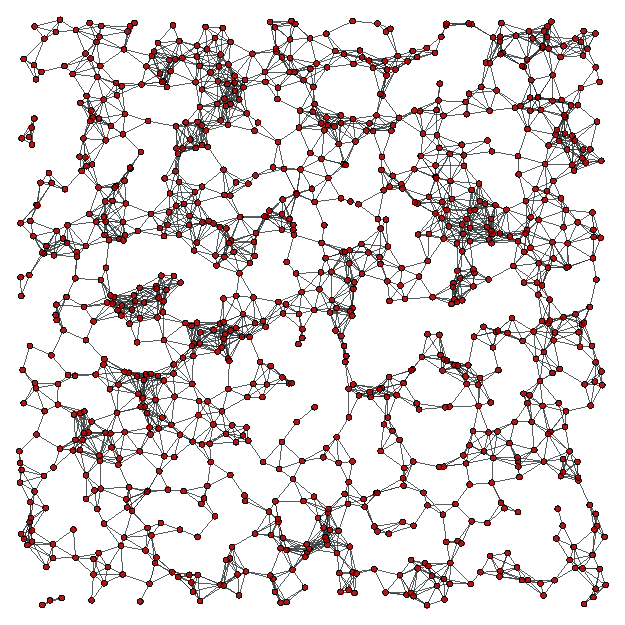
\includegraphics[scale=0.55]{./Figures/geometric.pdf}
\caption{Random geometric graph with 350 nodes and an edge for the pairs with an euclidean distance lower than 0.75.} \label{fig:GeoExample}
\end{figure}

To test if the coloring returned by the FrogSim algorithm is good, we look for the maximum \emph{$k$-clique}\footnote{A \emph{$k$-clique} being a subset of $k$ nodes having an edge between any pair of these nodes.} as such we know there is at least $k$ colors needed. A $8$-clique for the graph given at the Figure \ref{fig:GeoExample} is represented in red in the \ref{fig:GeoFullyConnected}.
\begin{figure}[h]
\centering
\includegraphics[scale=0.55]{./Figures/geo-sub_fully_connected.pdf}
\caption{Lower bound for the minimum number of colors needed (8).} \label{fig:GeoFullyConnected}
\end{figure}

\begin{figure}[h]
\centering
\includegraphics[scale=0.55]{./Figures/geo-coloried.pdf}
\caption{Instance of a valid coloring returned by the FrogSim algorithm.} \label{fig:GeoColoried}
\end{figure}


\subsubsection{Convergence Rate}
The algorithm specified by \cite{HB10} is designed to converge as fast as possible, depending on the parameter. We can see in the Figure \ref{fig:GeoPhaseConv0.5} and the Figure \ref{fig:GeoPhaseDynConv}, that the system get stable near the twentieth communication round. The need of convergence of the system can be explained in terms of getting an acceptable coloring in a minimum amount of communication rounds. Once the $\theta$-values do not change anymore, the colors do not change either.\\
First the algorithm is tested with the typical parameters specified by \cite{HB10}, ($\alpha = 0.5$). The resulting coloring are acceptable solutions where the number of colors is equal to the minimum possible or very close--usually $k^*$ or $k^*+1$.
\begin{figure}[h]
\centering
\includegraphics[scale=0.4]{./Figures/alpha_50.pdf}
\caption{Convergence of the $\theta$-values for the nodes of a clique.($\alpha_i = 0.5$)} \label{fig:GeoPhaseConv0.5}
\end{figure}

A second set of parameters have been tested. The second experiment take into account some remarks of \cite{HH12} and initialize the $\alpha$-values--the convergence--of the nodes according to the number of neighbors of each node. First, a convergence value is set for all the nodes of the system as an upper bound value. Then the value is changed, during the start message, according with the number of neighbors that a particular node get--which is denoted $n_i$.
\begin{equation}
\alpha_i = \alpha * 1-\frac{1}{\ln{n_i + 2}}
\end{equation}
This value is set as such in order to force the less influenced nodes to stabilize first. An example of the $\theta$-values comportment for a clique\footnote{This is interesting because a large clique will be composed of nodes that are highly influenced.} is shown in the Figure \ref{fig:GeoPhaseDynConv} and the evolution of the average $\theta$-values in the system is draw in the Figure \ref{fig:AvgDynConv}.
\begin{figure}[h]
\centering
\includegraphics[scale=0.4]{./Figures/dyn_conv.pdf}
\caption{Convergence of the $\theta$-values for the nodes of a clique for a specifier $\alpha$-value.} \label{fig:GeoPhaseDynConv}
\end{figure}

\begin{figure}[h]
\centering
\includegraphics[scale=0.4]{./Figures/phase_avg.pdf}
\caption{Average of the $\theta$-values for a system with specified a convergence value for each node.} \label{fig:AvgDynConv}
\end{figure}


\subsection{Grid topologies}
\label{subsec:gridtopology}
Graphs representing grid topologies have very similar look to a chessboard where each cell is a node and edges are present between adjacent cells. These graphs are essentially matrices where a link only exists between cells directly next to each other ; as such grid topologies have the same two dimensional parameters as matrices do. A grid topology graph will be classified following it's $n\times m$ dimensions.\\

An example of such a graph can be found in Figure ~\ref{fig:GridExample}.

\begin{figure}[h]
\centering
\includegraphics[]{./Figures/GridTopologyExample.pdf}
\caption{Example of a $4\times 3$ grid topology graph.} \label{fig:GridExample}
\end{figure}

Grid topologies are very easily colored theoretically and in centralized systems. This comes from the fact that all such graphs only ever need two colors. Indeed, as seen in Figure ~\ref{fig:GridExampleColored}, the optimal coloring is that of a chessboard : every other node is black and the nodes inbetween are white\footnote{Any other pair of colors can of course be used.}.

\begin{figure}[h]
\centering
\includegraphics[]{./Figures/GridTopologyExampleColored.pdf}
\caption{Optimally colorized Figure ~\ref{fig:GridExample} graph.} \label{fig:GridExampleColored}
\end{figure}

However, as ~\cite{HB10} discussed, distributed systems are unable to discover an optimal coloring as easily. Because each node only knows its direct neighbors, it is impossible for a node to know its exact position in the grid and as such to know what its optimal color should be. More complex algorithms are thus needed to find optimal coloring, such as \emph{FrogSim}.

\begin{figure}[h]
\centering
\includegraphics[scale=0.5]{./Figures/grid.pdf}
\caption{$10 \times 10$ grid.} \label{fig:GridInstance}
\end{figure}

\begin{figure}[h]
\centering
\includegraphics[scale=0.5]{./Figures/grid-coloration.pdf}
\caption{$10 \times 10$ grid coloring instances returned by FrogSim.} \label{fig:GridColoration}
\end{figure}

\subsubsection{Convergence Rate}
The algorithm takes more times to stabilize for the grid topology because of the influence--even indirect--of each node on all the other nodes of the system. As such the optimal coloring is much harder to achieve due to the unique solution. Similarly to any other topologies the algorithm should expand stability from the less influenced nodes, which in this case are the four corners of the grid. An example of $\theta$-values behaviour is shown at the Figure \ref{fig:GridConv}.

\begin{figure}[h]
\centering
\includegraphics[scale=0.4]{./Figures/grid_conv.pdf}
\caption{Evolution of the $\theta$-values for a $3 \times 3$ sub-graph of a grid.} \label{fig:GridConv}
\end{figure}

As a simple remark, the optimal solution has been returned for the grid topology after we made an error by initializing the convergence rate at $75$ instead of $0.75$. The comportment of the phase was a permanent switch between approximately 0 and 1.

\section{Discussion}

\subsection{Amelioration for Grid Topologies}
The discussed algorithm being a distributed heuristic that also uses the concept of spanning tree and master node of the graph to be colored can be optimized for graph representing a grid topology. In fact, when accepting the use of a master node in our distributed algorithm, we can easily build a deterministic algorithm that will achieve better performances.\\

We know that the optimal coloring of a grid topology is that of a chessboard\footnote{See Grid Topology on page ~\pageref{subsec:gridtopology}.}. The challenge to find such an optimal coloring with a distributed algorithm is that the nodes do not know their exact position within the grid : they only know their neighbors.\\

Because we accept the use of a master node, we can use the following algorithm to color the graph. Each node, starting with the master node, will broadcast to its neighbors a message containing its distance\footnote{The number of hops necessary to get to the master node from the current node.} from the master node. The nodes with an even distance from the master node will arbitrarily be colored black, and those with odd distance white. The messages will only be sent when the node is sure of its distance ; this happens when itself has received a message from a neighbor giving the neighbor's distance, from which the node can easily calculate its own distance : the neighbor's distance is simply incremented.\\

The algorithm starts with the master node sending a message containing $0$ to all its neighbors. all these neighbors now broadcast a $1$, and so on. When a node receives a message after having broadcasted its distance, the message is ignored.\\
In practice, the messages are broadcasted along the spanning tree of the graph which implies that the time for the algorithm to conclude is dependent on the height of said spanning tree ; it will take the time for $h$ successive message to be sent (and analyzed when received), where $h$ is the height of the spanning tree.\\

In a grid topology the spanning tree of minimal height $h^*$ has it's root in the middle of the grid. Say the grid has dimensions $n\times m$, $h^*$ can be found using the following formula :\\
\begin{center}$h^* = \lceil{\frac{max(m,n)}{2}}\rceil$\end{center}
$h^*$ is the total number of time steps required by this proposed algorithm to converge on the optimal coloration of the given graph representing a grid topology.

\footnotesize
\bibliographystyle{apalike}
\bibliography{report}

\end{document}
